% ============================================================================
% Resultados con julio y agosto de 2026 (secciones 8 y 9)
% Números de: modelo_sam/salidas/sistema/*.csv (script sistema_condicion.py)
% ============================================================================

\section{Calibración y verificación con julio y agosto de 2026}\label{sec:calibracion}\label{sec:resultados}

\subsection{Datos y criterio}
\enpalabras{La G-21 calibra; la 60-CH se evalúa. La G-21 tiene un protocolo municipal funcionando, y sus cierres reflejan una práctica que vale la pena reproducir. La 60-CH tiene un cierre binacional de 35 días que se quiere \emph{evaluar}. Si el modelo se calibrara con ella, aprendería ``así decide la autoridad'' en vez de ``así se comporta la cordillera''.}

\paragraph{Entradas.} ERA5-Land por tramo (nieve, lluvia, temperatura, manto), isoterma ERA5 y ráfagas ERA5 (\texttt{fg10}, 0,25°), agregadas en bloques de 6 h locales entre el 1 de julio y el 31 de agosto de 2026 (248 bloques por tramo).

\paragraph{Observado.} El estado de la ruta descrito en la sección~\ref{sec:contexto}, agrupado en tres clases: abierto; restringido o cierre técnico; cerrado por meteorología. Un bloque cuenta como cerrado si tuvo al menos una hora de cierre meteorológico. Los bloques ``cerrado por horario'' quedan fuera (capa administrativa).

\paragraph{El cuadro del protocolo de Lo Barnechea.} El cuadro se aplica de forma continua. Su nivel se calcula en cada hora con la nieve y la lluvia de las 12 horas anteriores y la isoterma media de esas horas, y el nivel del bloque es el más alto que alcanzó dentro de él. Ese nivel es también el piso de la regla híbrida.

\paragraph{Modelo en tres clases.} $E_0$ y $E_1$ cuentan como abierto (con o sin cadenas); $E_2$, como restricción fuerte o cierre parcial; $E_3$, $E_4$ y $E_5$, como cerrado.

\paragraph{Métricas.} Cinco números, cada uno con una pregunta. El kappa ponderado mide el acuerdo en las tres clases descontando el que daría el azar (1 es acuerdo perfecto; 0, el del azar) y castiga más confundir ``abierto'' con ``cerrado'' que con ``restricción''. Para la clase ``cerrado'': el POD dice qué fracción de los bloques cerrados detecta el modelo; el FAR, qué fracción de los cierres del modelo no ocurrió; el CSI, los aciertos sobre aciertos, falsas alarmas y omisiones; y el HSS, cuánto mejor que el azar acierta el modelo.

\subsection{Parámetros calibrados}
La calibración busca en una grilla la capacidad de despeje $c$ (0,5 a 8 cm/h), la nieve residual para reabrir $\theta$ (5 a 50 cm) y el umbral de peligro $H^\star$ (3, 4 o 5) que maximizan el kappa ponderado en la G-21 (cuadro~\ref{tab:calibracion}).

\begin{table}[H]
\centering\small
\caption{Parámetros calibrados con la G-21.}
\label{tab:calibracion}
\begin{tabular}{|l|c|l|}
\hline
Parámetro & Valor & Comentario \\ \hline
Umbral de peligro $H^\star$ & 5 & mejor kappa con 5 (0,54) que con 4 (0,45) o 3 (0,30) \\ \hline
Capacidad de despeje $c$ & 6 cm/h & cota inferior: el kappa sube hasta 6 cm/h y luego se aplana (fig.~\ref{fig:curva_c}) \\ \hline
Nieve residual para reabrir $\theta$ & 50 cm & con $c \ge 6$ el resultado casi no depende de $\theta$ \\ \hline
\end{tabular}
\end{table}

La G-21 acota la capacidad, no la fija. Bajo unos 4 cm/h el modelo mantiene cerrada la G-21 cuando en la realidad ya estaba abierta (kappa 0,46 con 2 cm/h); desde 6 cm/h el ajuste ya no mejora (0,54 con 6 y con 8 cm/h). Por eso el contrafactual de la sección~\ref{sec:contrafactual} se repite con tres capacidades.

\begin{figure}[H]
\centering
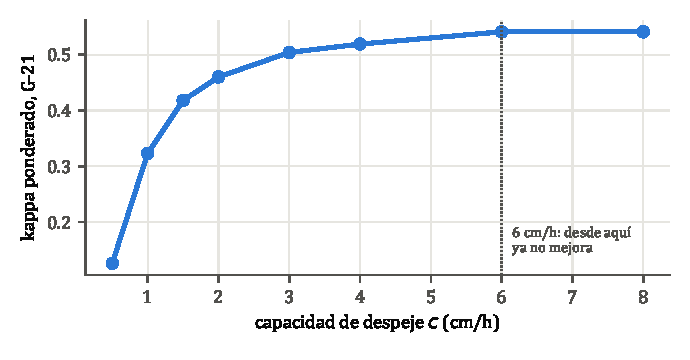
\includegraphics[width=0.62\textwidth]{fig/curva_capacidad.pdf}
\caption{Kappa ponderado de la G-21 según la capacidad de despeje. Con menos de unos 4 cm/h el modelo mantiene cerrada la G-21 cuando en la realidad ya estaba abierta; desde 6 cm/h el ajuste ya no mejora. La G-21 solo acota la capacidad por abajo.}
\label{fig:curva_c}
\end{figure}

\paragraph{Qué significa 6 cm/h en máquinas.} Con la ecuación~\eqref{eq:capacidad}, el tramo alto de la 60-CH ($\ell = 28{,}9$ km, $p = 2$ pasadas), una profundidad tolerada por pasada de $d = 10$ cm y una velocidad de avance de $s = 10$ km/h (valores ilustrativos, a confirmar con Vialidad), cada máquina aporta $c_1 = 10 \cdot 10 / (2 \cdot 28{,}9) \approx 1{,}7$ cm/h. Así, 6 cm/h equivalen a unas 3 o 4 máquinas trabajando a la vez en el tramo. El inventario de la 60-CH tiene 13 equipos activos de despeje: 4 cargadores frontales, 2 fresadoras de nieve, 5 bulldozers y 2 camiones con pala.

\subsection{Verificación: tres reglas y dos líneas base}

\begin{table}[H]
\centering\footnotesize\setlength{\tabcolsep}{4pt}
\caption{Verificación por bloque de 6 h. Kappa y exactitud en tres clases; POD, FAR, CSI y HSS para la clase ``cerrado''. G-21: 248 bloques, 19 cerrados. 60-CH: 212 bloques (sin los cerrados por horario), 176 cerrados. El cuadro del protocolo de Lo Barnechea usa solo sus gatillantes de nieve, lluvia e isoterma, con el nivel horario más alto de cada bloque; en la 60-CH se aplica como referencia, porque ese protocolo no rige ahí.}
\label{tab:metricas}
\begin{tabular}{|l|l|c|c|c|c|c|c|}
\hline
Modelo & Ruta & Exactitud & Kappa & POD & FAR & CSI & HSS \\ \hline
(A) Híbrida (propuesta) & G-21 & 0,79 & 0,54 & 0,68 & 0,46 & 0,43 & 0,57 \\ \hline
(A) Híbrida (propuesta) & 60-CH & 0,47 & 0,21 & 0,41 & 0,00 & 0,41 & 0,19 \\ \hline
(B) Walker pura & G-21 & 0,91 & 0,63 & 0,68 & 0,41 & 0,46 & 0,60 \\ \hline
(B) Walker pura & 60-CH & 0,47 & 0,17 & 0,41 & 0,00 & 0,41 & 0,19 \\ \hline
(C) Peligro dentro de la severidad & G-21 & 0,77 & 0,41 & 0,21 & 0,33 & 0,19 & 0,29 \\ \hline
(C) Peligro dentro de la severidad & 60-CH & 0,14 & 0,05 & 0,01 & 0,00 & 0,01 & 0,00 \\ \hline
Protocolo de Lo Barnechea (cuadro) & G-21 & 0,79 & 0,27 & 0,00 & 1,00 & 0,00 & $-$0,02 \\ \hline
Protocolo de Lo Barnechea (cuadro) & 60-CH & 0,14 & 0,04 & 0,01 & 0,00 & 0,01 & 0,00 \\ \hline
Persistencia (estado observado 6 h antes) & G-21 & 0,98 & 0,93 & 0,95 & 0,05 & 0,90 & 0,94 \\ \hline
Persistencia (estado observado 6 h antes) & 60-CH & 0,97 & 0,84 & 0,98 & 0,02 & 0,97 & 0,82 \\ \hline
\end{tabular}
\end{table}

\paragraph{El sistema frente al protocolo de Lo Barnechea.} El sistema ve los cierres que el cuadro no ve. Aplicado de forma continua, ese cuadro no detecta ningún cierre de la G-21 (POD 0) y da dos falsas alarmas, ambas el 8 de agosto. El sistema detecta 13 de los 19 bloques cerrados (kappa 0,54 contra 0,27).

\paragraph{El corte del 17 al 20 de julio.} El sistema justifica el corte, pero por otro mecanismo. La Resolución Exenta N.º 4.172 de la Dirección de Vialidad cortó la G-21 entre los kilómetros 1 y 36,3 por desprendimiento de rodados y acumulación de nieve; ese mismo día, un aluvión del río Ñilhue sobrepasó las mallas de contención entre los kilómetros 6 y 6,5. El sistema clasifica como cierre por peligro ($E_5$) 10 de los 11 bloques del corte, sin ver el estado observado, y la duración modelada se aparta de la observada en +1 y +7 horas (cuadro~\ref{tab:episodios}). Ese cierre, sin embargo, proviene del peligro de avalancha en el tramo alto (nota 5, con unos 35 cm de nieve en 12 h en la celda), mientras que el índice de remoción en masa del tramo medio, donde ocurrió el aluvión, no superó 2 de 5 (lluvia de 72 h de hasta 33 mm). El sistema no detectó el aluvión: el índice de remoción solo mira la lluvia de 72 horas y no ve la activación de quebradas.

\paragraph{El peligro aparte.} Diluido en un promedio, el peligro no pesa. Con la regla C el sistema cierra la 60-CH en 1 de sus 176 bloques cerrados y pierde la mayor parte de los cierres de la G-21 (POD 0,21). Separarlo no es una preferencia de diseño: es lo que permite justificar el cierre del 17 al 20 de julio.

\paragraph{Híbrida o Walker pura.} En la G-21 gana Walker pura, y la causa son dos reglas del protocolo de Lo Barnechea que entran por el piso (kappa 0,63 contra 0,54). Primero, en 34 bloques en que la G-21 estaba abierta, la híbrida marca cierre parcial porque el cuadro manda a Alerta 2 la ``presencia de precipitación líquida'' (50 de los 58 casos por tramo, todos con isoterma sobre 2.800 m). Segundo, el 8 de agosto la híbrida marca cierre total en dos bloques porque el cuadro exige Alerta 3 con más de 1 cm de nieve cuando la isoterma está entre 900 y 1.500 m: con 1,15 cm en 12 h e isoterma de 1.407 m, la G-21 estaba abierta. En la 60-CH la híbrida queda algo arriba (0,21 contra 0,17). La elección es de criterio. La híbrida garantiza cumplir ese protocolo; Walker pura se acerca más a lo que la práctica hace con la lluvia y con las nevadas mínimas. Hay una tercera vía: mantener la híbrida y revisar esas dos reglas en el cuadro de Lo Barnechea.

\paragraph{La persistencia.} La persistencia gana, pero juega otro partido. Repetir el estado de 6 horas antes acierta casi siempre (kappa 0,93 en la G-21), porque los estados duran muchos bloques. El sistema no mira el estado observado: todo sale de la meteorología. La persistencia sirve para el día a día, pero no dice si un cierre está justificado ni sirve en rutas sin historial.

\paragraph{La 60-CH.} En la 60-CH el bajo kappa es el resultado, no el error. Cuando el sistema cierra la 60-CH, el camino estaba cerrado (FAR 0). Lo que no reproduce es la duración: la mayor parte de las horas que la 60-CH estuvo cerrada, el sistema la considera transitable con restricción. La sección~\ref{sec:contrafactual} analiza esa diferencia.

\begin{figure}[p]
\centering
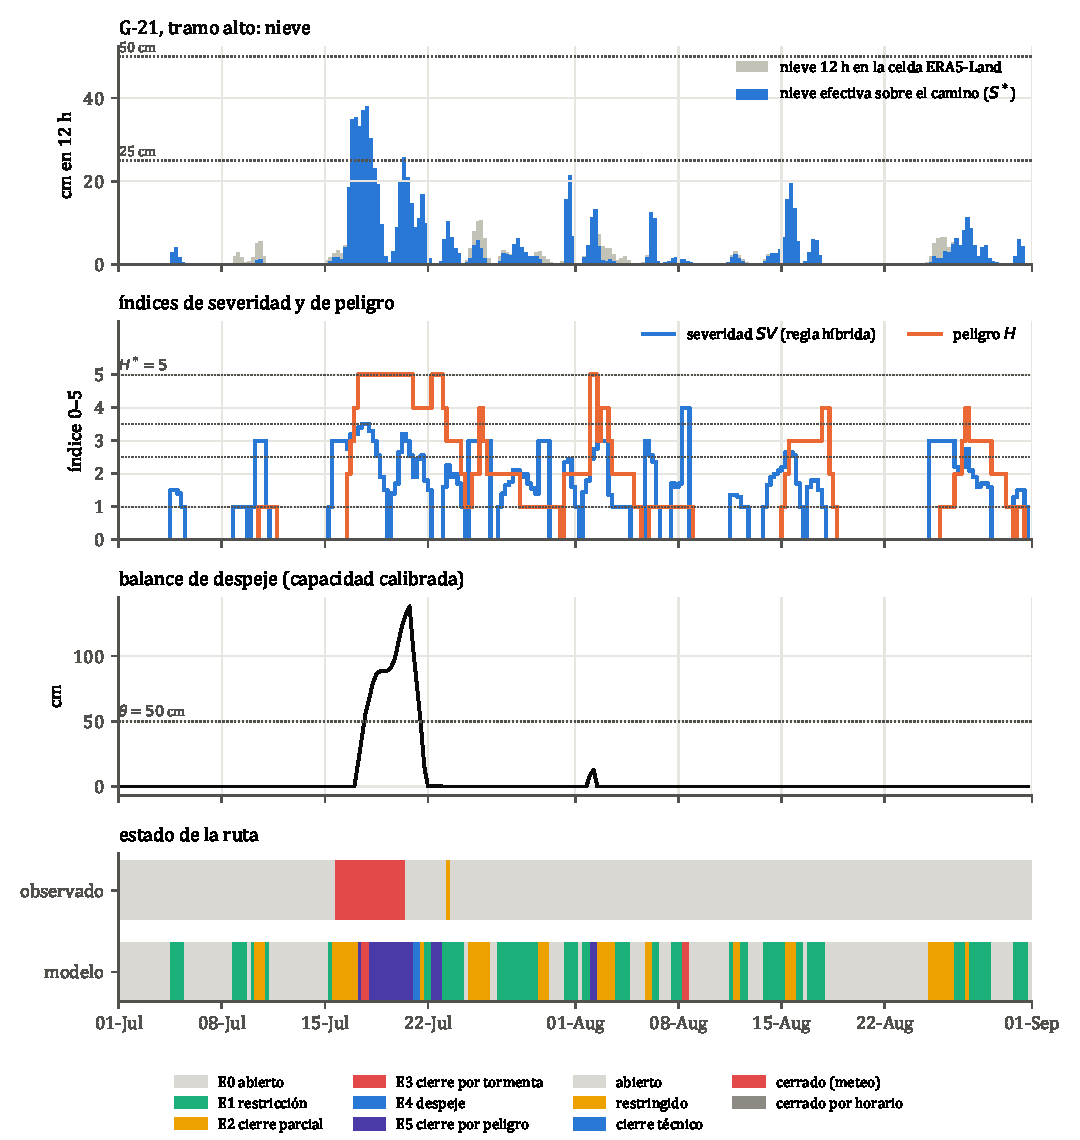
\includegraphics[width=\textwidth]{fig/serie_G21.pdf}
\caption{G-21, tramo alto. Arriba: nieve en 12 h en la celda ERA5-Land y nieve efectiva sobre el camino. Al medio: índices de severidad y de peligro, y balance de despeje. Abajo: estado observado de la ruta y estado del modelo (tramo en peor condición). El cierre de julio (tormenta, rodados y aluvión del río Ñilhue) cae en $E_3$ y $E_5$, con el peligro de avalancha del tramo alto; el resto del periodo el modelo marca sobre todo abierto o restricción.}
\label{fig:serieG21}
\end{figure}

\begin{table}[H]
\centering\footnotesize\setlength{\tabcolsep}{4pt}
\caption{Episodios de cierre meteorológico observados y lo que dice el modelo (capacidad calibrada). Bloques de 6 h en cada estado; ``h modelo'' son las horas que el modelo considera cerrado ($E_3$, $E_4$ o $E_5$).}
\label{tab:episodios}
\begin{tabular}{|l|l|r|r|r|r|r|r|r|r|}
\hline
Ruta & Episodio & h obs. & $E_0$ & $E_1$ & $E_2$ & $E_3$ & $E_4$ & $E_5$ & h modelo \\ \hline
G-21 & 15/07 23h -- 17/07 18h (lluvia y nieve) & 43 & 0 & 0 & 6 & 2 & 0 & 1 & 18 \\ \hline
G-21 & 17/07 18h -- 19/07 11h (rodados, nieve, aluvión) & 41 & 0 & 0 & 0 & 1 & 0 & 6 & 42 \\ \hline
G-21 & 19/07 17h -- 20/07 10h (rodados, nieve, aluvión) & 17 & 0 & 0 & 0 & 0 & 0 & 4 & 24 \\ \hline
60-CH & 09/07 17h -- 11/07 11h & 42 & 0 & 5 & 3 & 0 & 0 & 0 & 0 \\ \hline
60-CH & 14/07 15h -- 18/08 08h & 833 & 24 & 42 & 9 & 1 & 10 & 54 & 390 \\ \hline
60-CH & 24/08 17h -- 29/08 09h & 112 & 2 & 4 & 7 & 0 & 0 & 7 & 42 \\ \hline
60-CH & 29/08 17h -- 30/08 08h & 15 & 3 & 1 & 0 & 0 & 0 & 0 & 0 \\ \hline
60-CH & 30/08 17h -- 31/08 10h & 17 & 1 & 3 & 0 & 0 & 0 & 0 & 0 \\ \hline
\end{tabular}
\end{table}

\paragraph{Los episodios.} En la G-21 el sistema acierta el corte del 17 al 20 de julio, por peligro de avalancha y no por el aluvión, y se queda corto en el cierre preventivo. El cierre del 15 al 17 de julio se decretó por ``alarma de precipitaciones intensas'' (43 h); el sistema lo ve como cierre parcial casi todo el tiempo y solo cierra 18 h. En la 60-CH, el episodio del 9 al 11 de julio no tiene respaldo en ningún bloque: la isoterma media del 10 de julio estuvo en 3.280 m, así que la línea de nieve quedó cerca de los 3.000 m y la nevada apenas tocó el camino.

\subsection{Capa estadística: logit ordinal}
\enpalabras{Sobre las reglas cabe una capa estadística pequeña. Toma los tres números del sistema (severidad, peligro y nieve por despejar) y los convierte en probabilidades de ``abierto'', ``restricción'' o ``cerrado''. Se ajusta con la G-21. Aplicada a la 60-CH, responde qué habría decidido un operador que cerrara como se cierra la G-21.}

El modelo es un logit ordinal (de odds proporcionales):
\begin{equation}
P(Y_t \le j) = \frac{1}{1 + \exp\!\big(-(\alpha_j - \beta_{SV}\, \widetilde{SV}_t - \beta_H\, \widetilde{H}_t - \beta_N\, \widetilde{N}_t)\big)}, \qquad j \in \{0, 1\},
\end{equation}
con las variables estandarizadas, $Y_t$ la clase observada (0 abierto, 1 restricción, 2 cerrado) y una penalización ridge leve por los pocos cierres. Los coeficientes estandarizados ($\beta_{SV} = 1{,}31$, $\beta_H = 0{,}75$, $\beta_N = 0{,}55$) son los tres positivos, como se espera. En la G-21 alcanza kappa 0,57 (POD 0,53, FAR 0,29).

\paragraph{Qué significa en horas.} De las 1.019 horas que la 60-CH estuvo cerrada por meteorología, el criterio aprendido en la G-21 habría cerrado 288 (28\,\%). Así, un operador ``como el de la G-21'' habría mantenido la ruta abierta, con o sin restricción, las otras 731 horas. Probabilidad media de cierre en esas horas: 0,31.

% ============================================================================
\section{El cierre largo de la 60-CH: ¿había otras opciones?}\label{sec:contrafactual}

\enpalabras{La pregunta no es si la autoridad se equivocó. Es qué parte del cierre tiene respaldo en la condición física del camino. Para cada bloque cerrado, el sistema dice qué estado justifica la meteorología: ``cierre por tormenta'', ``por peligro'', ``despejando'', ``cierre parcial'', ``restricción'' o nada. La capacidad de despeje es incierta, así que el cálculo se repite con tres capacidades.}

\begin{figure}[H]
\centering
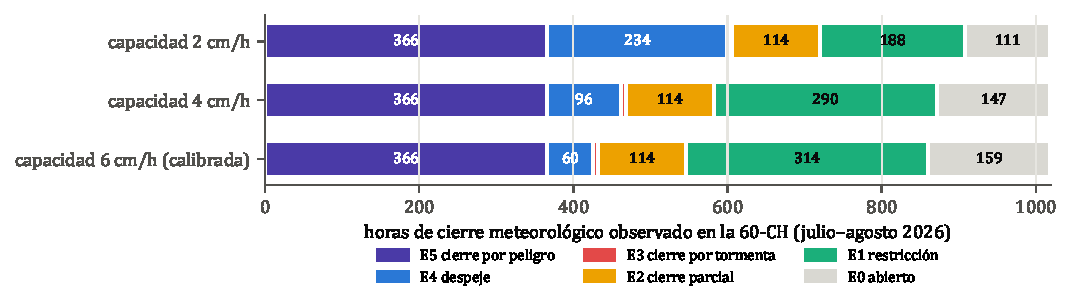
\includegraphics[width=\textwidth]{fig/contrafactual_60CH.pdf}
\caption{Las 1.019 horas de cierre meteorológico observado en la 60-CH (julio y agosto de 2026), según el estado que el sistema considera justificado, con tres capacidades de despeje. Las horas por peligro no dependen de la capacidad, porque con peligro alto no se despeja.}
\label{fig:contrafactual}
\end{figure}

\begin{table}[H]
\centering\footnotesize\setlength{\tabcolsep}{4pt}
\caption{Horas de cierre meteorológico observado en la 60-CH según el estado del modelo. ``Con respaldo'': el sistema justifica cierre total ($E_3$, $E_4$ o $E_5$). ``Sin respaldo'': justifica, como máximo, cierre parcial o restricción.}
\label{tab:contrafactual}
\begin{tabular}{|l|r|r|r|r|r|r|r|r|}
\hline
Capacidad & $E_5$ peligro & $E_3$ tormenta & $E_4$ despeje & $E_2$ parcial & $E_1$ restricción & $E_0$ abierto & Con respaldo & Sin respaldo \\ \hline
2 cm/h & 366 & 6 & 234 & 114 & 188 & 111 & 606 (59\,\%) & 413 (41\,\%) \\ \hline
4 cm/h & 366 & 6 & 96 & 114 & 290 & 147 & 468 (46\,\%) & 551 (54\,\%) \\ \hline
6 cm/h (calibrada) & 366 & 6 & 60 & 114 & 314 & 159 & 432 (42\,\%) & 587 (58\,\%) \\ \hline
\end{tabular}
\end{table}

\paragraph{La tormenta y el peligro.} La tormenta, por sí sola, casi nunca justificó cerrar la 60-CH; el peligro sí. Un solo bloque llega a $E_3$ (6 horas, el 17 de julio desde las 18:00), y lo hace por el piso del protocolo de Lo Barnechea: entre las 19:00 y las 22:00 la nieve de 12 h en la celda del tramo alto superó los 50 cm (hasta 51,6 cm), con isoterma cercana a 2.400 m, y el cuadro pasó a Alerta 3. En el resto, la nieve efectiva del tramo alto casi nunca supera los 40 cm en 12 h, porque la isoterma media diaria se mantuvo entre 2.100 y 3.600 m y solo una parte del camino quedó bajo nieve ($\varphi$ mediana de 0,38). Las 366 horas por peligro son las mismas con cualquier capacidad: con peligro alto no se despeja.

\paragraph{Día a día.} Entre el 14 de julio y el 18 de agosto (36 días, capacidad calibrada, estado más grave del día), el sistema da: 20 días con respaldo para cierre total, 19 por peligro de avalancha (16--23 y 25--30 de julio, 1--3 y 16--17 de agosto) y uno de despeje (24 de julio); 3 días de cierre parcial (15 de julio y 13--14 de agosto); 9 días de restricción con cadenas (31 de julio, 4--8, 11--12 y 15 de agosto); 4 días sin restricción meteorológica (14 de julio, 9--10 y 18 de agosto). Los días con respaldo coinciden con la gran tormenta de julio (unos 280 cm entre el 16 y el 21 en la celda ERA5-Land) y con las nevadas que siguieron sobre un manto que llegó a 2,3 m. El 14 de julio, el cierre se decretó con pronóstico, antes de que nevara.

\paragraph{La ventana del 4 al 12 de agosto.} Nueve días seguidos en que el sistema solo justifica restricción o apertura. Se leen en dos partes. Del 5 al 8 hubo poca nieve nueva (hasta 14 cm en 12 h en la celda, 9 cm efectivos), pero ráfagas de 25 a 31 m/s: viento blanco, que levanta la nieve y baja la visibilidad, un gatillante del protocolo de Lo Barnechea (Alerta 3 bajo 20 m) que ERA5 no entrega. Esos días pueden tener una justificación que el sistema no ve. Del 9 al 12, la nieve nueva de 72 h bajó a entre 3 y 15 cm, las ráfagas a entre 13 y 20 m/s, el peligro a 0 o 1 y el balance quedó en cero. Son los días con menos respaldo para el cierre total: el sistema indica que la ruta podía operar con restricción.

\paragraph{Qué se puede afirmar y qué no.} Con la calibración de la G-21, entre el 41\,\% y el 58\,\% de las horas de cierre de la 60-CH no tienen respaldo meteorológico para cierre total, según la capacidad de despeje. Un 11\,\% adicional justificaba solo cierre parcial. Esto no prueba que la decisión haya sido errada. Primero, el sistema no ve el lado argentino del paso, la visibilidad ni las evaluaciones de avalancha en terreno. Segundo, el resultado depende sobre todo de un supuesto: la exposición del tramo alto a avalanchas. Lo que sí muestra es que había opciones intermedias, que el protocolo de Lo Barnechea no contempla: cierre por peligro con ventanas de despeje, cierre parcial y restricción con cadenas. Y muestra qué dato falta para decidir mejor: un catastro de trayectorias de avalancha del tramo Juncal--Portillo--Los Libertadores.

\begin{figure}[p]
\centering
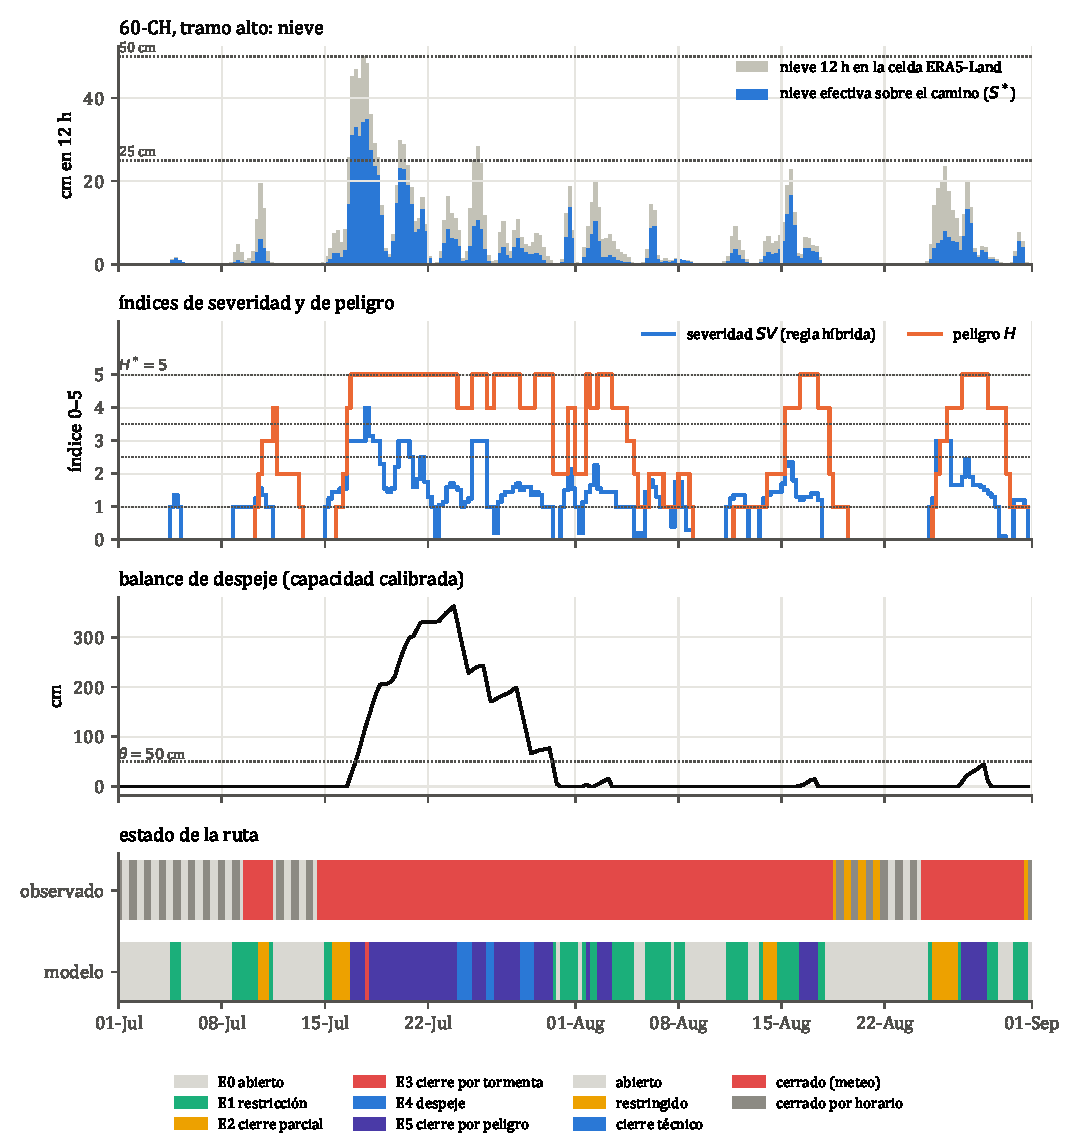
\includegraphics[width=\textwidth]{fig/serie_60CH.pdf}
\caption{60-CH, tramo alto, con la misma organización que la figura~\ref{fig:serieG21}. El cierre observado (rojo) se mantiene del 14 de julio al 18 de agosto. El modelo lo respalda con peligro ($E_5$) y despeje ($E_4$) hasta comienzos de agosto; luego pasa a restricción ($E_1$) y apertura ($E_0$), salvo un repunte de peligro el 16 y 17 de agosto. La nieve por despejar crece hasta unos 350 cm porque, con peligro alto, las cuadrillas no trabajan.}
\label{fig:serie60CH}
\end{figure}
